\begin{figure*}
\begin{subfigure}{0.34\textwidth}
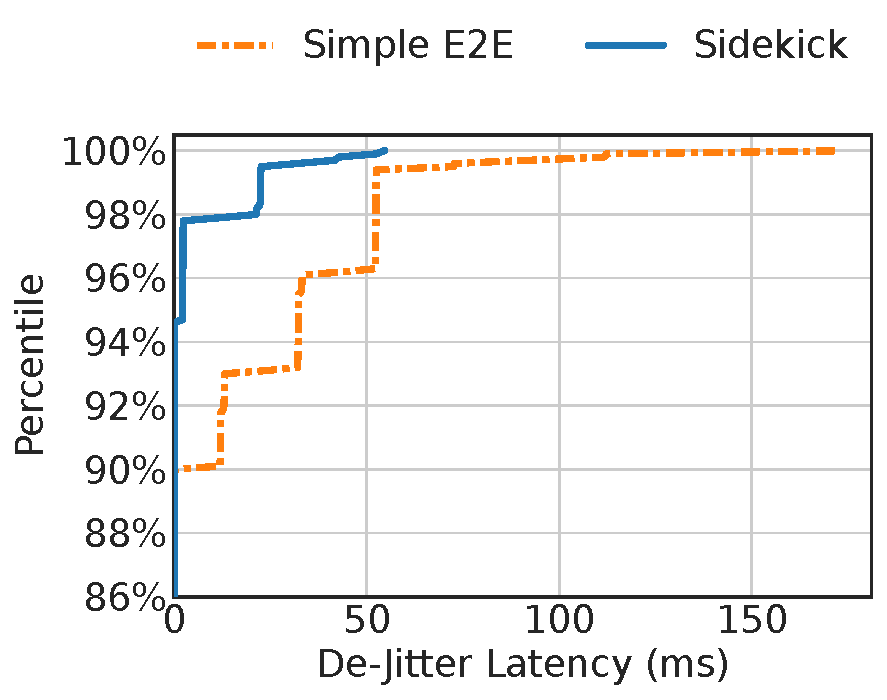
\includegraphics[width=\linewidth]{sidekick-paper/figures/fig4a_low_latency_media.pdf}
\caption{Scenario \#1: Low-latency media.
 Reduced tail latency of de-jitter delay
with earlier retransmission. 5 minute trials.}
\label{fig:media}
\end{subfigure}
\hfill
\begin{subfigure}{0.31\textwidth}
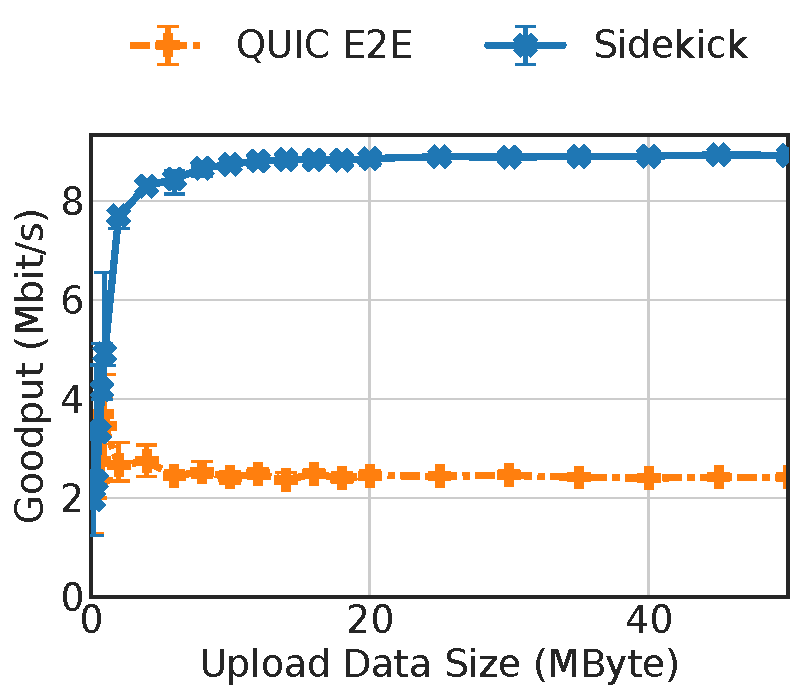
\includegraphics[width=0.97\linewidth]{sidekick-paper/figures/fig4b_pep_emulation.pdf}
\caption{Scenario \#2: Connection-splitting PEP emulation. Improved goodput.
20 trials median. Error bars are 1st and 3rd quartiles.
}
\label{fig:baseline-line}
\end{subfigure}
\hfill
\begin{subfigure}{0.32\textwidth}
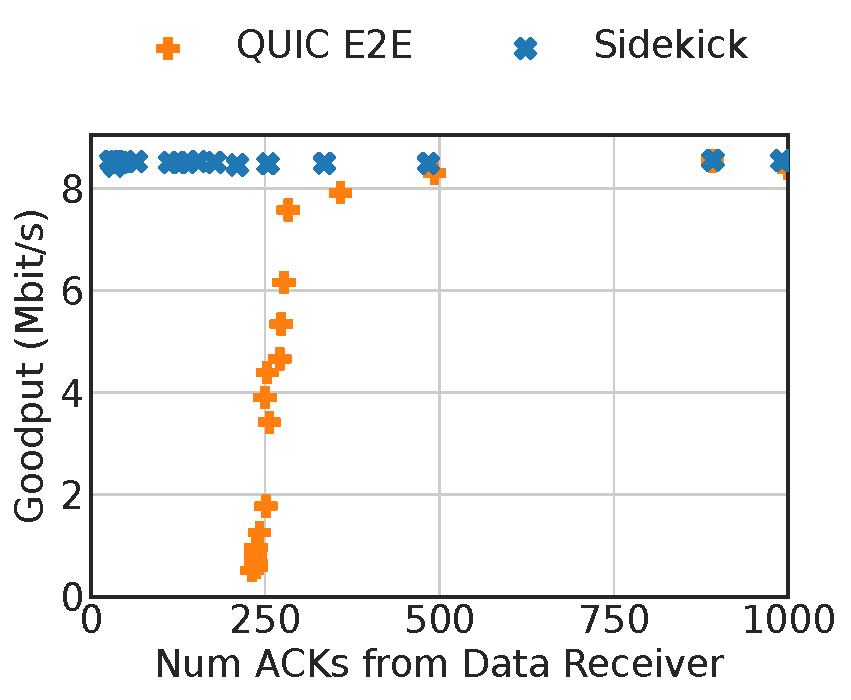
\includegraphics[width=0.99\linewidth]{sidekick-paper/figures/fig4c_ack_reduction.pdf}
\caption{Scenario \#3: ACK reduction.
High goodput independent of end-to-end ACK frequency.
10 MB upload.}
\label{fig:ack-reduction}
\end{subfigure}
\caption{
Comparing the end-to-end baseline protocol to the same protocol with a sidekick
connection, using the success metrics for the three scenarios described in
\Cref{tab:experimental-scenarios}. The \textsf{Sidekick($N$x)} data points show
the performance at $N$x the quACK interval (sent less frequently) and
threshold of the default configurations specified in
\Cref{tab:experimental-scenarios}.
\vspace{-0.3cm}
}
% \dm{Maybe a notation like $x/4$ would be more suggestive than $4x$?}
\label{fig:main-results}
\end{figure*}
